\newsavebox{\listA}
\newsavebox{\listB}

\lstset{language=myasm,style=smaller,morekeywords={decq}}
\begin{lrbox}{\listA}
\begin{minipage}{0.45\textwidth}
\lstinputlisting{../intro/perf-examples1.s}
\end{minipage}
\end{lrbox}
\lstset{language=myasm,style=smaller,morekeywords={decq}}
\begin{lrbox}{\listB}
\begin{minipage}{0.45\textwidth}
\lstinputlisting{../intro/perf-examples2.s}
\end{minipage}
\end{lrbox}

\begin{frame}
\frametitle{some performance examples}
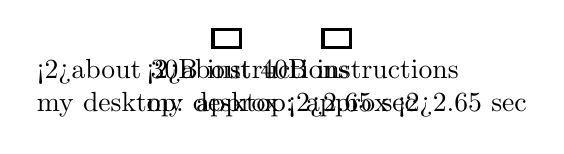
\begin{tikzpicture}
\node[draw,very thick,align=left] (v1) {
\usebox{\listA}
};
\node[align=left,anchor=north] at (v1.south) {
\myemph<2>{about 30B} instructions \\
my desktop: approx \myemph<2>{2.65 sec}
};
\node[align=left,draw,very thick,anchor=north west] (v2) at ([xshift=1cm]v1.north east) {
\usebox{\listB}
};
\node[align=left,anchor=north] at (v2.south) {
\myemph<2>{about 40B} instructions \\
my desktop: approx \myemph<2>{2.65 sec}
};
\end{tikzpicture}
\end{frame}
